
\documentclass[DIV=calc,paper=a4,fontsize=9pt,twocolumn]{scrartcl}
\renewcommand*\sfdefault{lcmss}
\renewcommand*\familydefault{\sfdefault} 
\usepackage[T1]{fontenc}

\usepackage{lipsum}         
\usepackage{eurosym}
\usepackage[utf8]{inputenc}
\usepackage[german]{babel}								
\usepackage[protrusion=true,expansion=true]{microtype}	
\usepackage{amsmath,amsfonts,amsthm}					
\usepackage[pdftex]{graphicx}							
\usepackage[svgnames]{xcolor}							

\usepackage{epstopdf}									
\usepackage{subfig}										
\usepackage{booktabs}									
\usepackage{fix-cm}										
\usepackage{csquotes}
\usepackage[authoryear,round]{natbib}
\usepackage{float}
\usepackage{url}
\bibliographystyle{apalike}
\definecolor{headblue}{HTML}{15778E}
\definecolor{borderblue}{HTML}{074C5C}

\usepackage{listings}

\usepackage{color}
\definecolor{gray}{rgb}{0.4,0.4,0.4}
\definecolor{darkblue}{rgb}{0.0,0.0,0.6}
\definecolor{cyan}{rgb}{0.0,0.6,0.6}

\lstset{
  basicstyle=\ttfamily,
  columns=fullflexible,
  showstringspaces=false,
  commentstyle=\color{gray}\upshape
}

\lstdefinelanguage{XML}
{
  morestring=[b]",
  morestring=[s]{>}{<},
  morecomment=[s]{<?}{?>},
  stringstyle=\color{black},
  identifierstyle=\color{darkblue},
  keywordstyle=\color{cyan},
  morekeywords={xmlns,version,type}% list your attributes here
}


\usepackage{sectsty}		
							
\allsectionsfont{\usefont{OT1}{phv}{b}{n}}				
														

\sectionfont{\usefont{OT1}{phv}{b}{n}}					
														




\usepackage{fancyhdr}									
    \pagestyle{fancy}									
\usepackage{lastpage}   


\lhead{}
\chead{}
\rhead{}

\lfoot{\footnotesize 2014 \textbullet ~ DBW: Datenbanken und Wissensrepräsentationen - Praktikum 1}
\cfoot{}
\rfoot{\footnotesize Seite \thepage\ von \pageref{LastPage}}  
\renewcommand{\headrulewidth}{0.0pt}
\renewcommand{\footrulewidth}{0.4pt}




\usepackage{lettrine}
\newcommand{\initial}[1]{
     \lettrine[lines=2,lhang=0.3,nindent=0em]{
                    \color{headblue}
                    {\textsf{#1}}}{}}




\usepackage{titling}										

\newcommand{\HorRule}{\color{headblue}\rule{\linewidth}{1pt}}

\pretitle{\vspace{-30pt} \begin{flushleft}  \fontsize{30}{30} \usefont{OT1}{phv}{b}{n} \color{borderblue} \selectfont }
\title{DBW: Datenbanken und Wissensrepräsentationen - Praktikum 1}    
\posttitle{\par\end{flushleft}\vskip 0.5em}

\preauthor{\begin{flushleft} \large \usefont{OT1}{phv}{b}{sl} \color{headblue}}
\author{Steffen Tröster - 11075591\\}											
\postauthor{\footnotesize \usefont{OT1}{phv}{m}{sl} \color{Black} 
                    Fachhochschule Köln, April 2014
                    \par\end{flushleft}\HorRule}

\date{}																




\begin{document}
\maketitle
\thispagestyle{fancy}		
\initial{D}as erste Praktikum des Moduls Datenbanken und Wissensrepräsentationen beschäftigt sich mit formalen Wissensrepräsentationen am Beispiel von XML und die somit mögliche Überfürhung zur Speicherung dieser Informationen. Dabei wird zunächst ein exmplarisches Wissensgebiet gewählt, näher beschrieben, strukturiert und es werden Beispiele für die verschiedensten Wissensformen dargelegt. 

\section{Das Wissensgebiet - Unternehmen}

Das in diesem Praktikum gewähle Wissensgebiet soll eine grobe Darstellung der Struktur eines mittelständigen Unternehmens sein. Der Anspruch einer vollständigen Abbildung des Gebiets ist nicht erhoben. Im folgenden wird Wissen als Faktenwissen, Regelwissen und Einschränkungen (o.a. Constraints) zu dem Wissensgebiet eingeordnet.

\subsection{Faktenwissen}
\begin{itemize}
    \item Frank Müller arbeitet in dem Unternehmen \enquote{transfluid} in der Verwaltung als Buchhalter.
    \item Die Abteilung der Buchhaltung wird von Herrn Schmidt geleitet, er ist zudem auch geschäftsführender Leiter des Unternehmens.
    \item Das Unternehmen stellt den Staubsauger \enquote{Saugermax 250} her. Dieser Staubsauger kostet 320,50 \euro .
    \item Für einen \enquote{Saugermax 250} benötigen die Mitarbeiter 7 Stunden.
    \item Bei der Herstellung des \enquote{Saugermax 250} bleibt er eine Stunde in der Testabteilung.
    \item Stratman Elektronik aus Köln beliefert das Unternehmen \enquote{transfluid} , sie liefern Platinen.
\end{itemize}

\subsection{Relationswissen und Regelwissen}

\begin{itemize}
    \item Mitarbeiter arbeiten in einem Unternehmen.
    \item In Abteilungen sind mehrere Mitarbeiter beschäftigt.
    \item Das Unternehmen ist in Abteilungen unterteilt.
    \item Im Unternehmen werden Produkte hergestellt.
    \item Produkte werden von Mitarbeitern gefertigt.
    \item Das Produkt durchläuft während der Produktion mehrere Abteilungen.
    \item Eine Abteilung wird von mehreren Produkten durchlaufen.
    \item Ein Unternehmen hat mehrere Zulieferer.
    \item Ein Mitarbeiter verhandelt mit den Zulieferern.
    \item Ein Teil kann von unterschiedlichen Zulieferern geliefert werden.
    \item Die Teile werden zur Fertigung eines Produktes benötigt.
    \item Ein Produkt benötigt mehrere Teile.
\end{itemize}


\subsection{Constraints}

\begin{itemize}
\item Es gibt nur einen Abteilungsleiter je Abteilung
\item Abteilungsleiter können immer nur eine Abteilung leiten.
\item Ein Mitarbeiter kann nicht gleichzeitig in mehreren Abteilungen beschäftigt sein.
\item Ein Zulieferer hat genau einen Mitarbeiter als Ansprechpartner im Unternehmen.
\end{itemize}

\section{Modellierung}

Aus den beispielhaften Wissensangaben soll nun ein Relationales Entitätenmodell erstellt werden. Nach Betrachtung aller Angaben konnten folgende Entitäten identifiziert werden: Unternehmen, Mitarbeiter, Abteilung, Produkt, Teile. Aus diesen Entitäten und den Relationen aus dem Regelwissen und Constrains ist das in Abbildung \ref{fig:er} abgebildete ER-Modell entstanden.

\begin{figure*}[ht]
    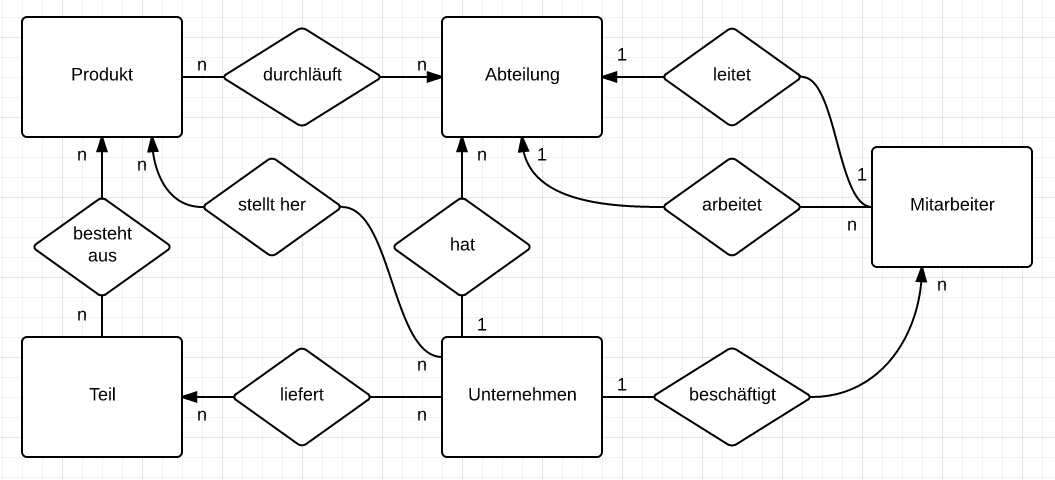
\includegraphics[width=0.95\textwidth ]{er.png}{}
    \centering
    \caption{ER-Modell des Wissensgebiets Unternehmen}\label{fig:er}
\end{figure*}

\subsection{XML Definition}

Aus zwei Entitäten sollen nun exemplarische XML Dokumente erstellt werden, die von einem später zu implementierenden Java Programm geparst werden sollen. Es wurde sich hier für die beiden Entitäten Mitarbeiter und Produkt entschieden, die dabei die folgenden Attribute erhalten sollen:

\begin{itemize}
\item Mitarbeiter (ID, Name, Abteilung, Wohnort, Gehalt) 
\item Produkt (ID, Name, Bauzeit, Preis) 
\end{itemize}

Hierbei ist für die Entitäten Produkt und Mitarbeiter sind folgendes XML Dokumente mit darauf folgenden XSDs entstanden:

\subsubsection{Produkt XML Dokument}

\lstset{language=XML}
\begin{lstlisting}
<?xml version="1.0" encoding="UTF-8"?>
<products xsi:noNamespaceSchemaLocation="products.xsd"
xmlns:xsi="http://www.w3.org/2001/XMLSchema-instance">
    <product id="0">
        <name>Staubmax 250</name>
        <buildtime>07:45:34</buildtime>
        <price current="euro">12.50</price>
    </product>
    <product id="1">
        <name>Staubmax 230i</name>
        <buildtime>07:05:34</buildtime>
        <price current="euro">14.50</price>
    </product>
</products>
\end{lstlisting}

\subsubsection{Mitarbeiter XML Dokument}

\lstset{language=XML}
\begin{lstlisting}
<?xml version="1.0" encoding="UTF-8"?>
<employees xsi:noNamespaceSchemaLocation="employees.xsd"
xmlns:xsi="http://www.w3.org/2001/XMLSchema-instance">
    <employee id="12">
        <name>Steffen Troester</name>
        <department id="23" leading="false">
            Softwareentwicklung
        </department>
        <payment current="euro">2100</payment>
        <hometown>Wormbach</hometown>
    </employee>
    <employee id="13">
        <name>Bernd Schneider</name>
        <department id="24" leading="true">
            Management
        </department>
        <payment current="euro">3100</payment>
        <hometown>Koeln</hometown>
    </employee>
</employees>
\end{lstlisting}

\subsubsection{Produkt XSD Schema Dokument}

\lstset{language=XML}
\begin{lstlisting}
<?xml version="1.0" encoding="UTF-8"?>
<xs:schema version="1.0"
xmlns:xs="http://www.w3.org/2001/XMLSchema">
    <xs:element name="products">
        <xs:complexType>
            <xs:sequence>
                <xs:element name="product" 
                maxOccurs="unbounded" type="product">
                </xs:element>
            </xs:sequence>
        </xs:complexType>
    </xs:element>

    <xs:complexType name="product">
        <xs:sequence>
            <xs:element name="name" type="xs:string"/>
            <xs:element name="buildtime" type="buildtime"/>
            <xs:element name="price" type="price"/>
        </xs:sequence>
        <xs:attribute name="id" type="xs:int"/>
    </xs:complexType>

    <xs:simpleType name="buildtime">
        <xs:restriction base="xs:string">
            <xs:pattern value="[0-9]{2}:[0-9]{2}:[0-9]{2}"/>
        </xs:restriction>
    </xs:simpleType>

    <xs:complexType name="price">
        <xs:simpleContent>
            <xs:extension base="xs:float">
                <xs:attribute name="current" 
                type="currenttype"/>
            </xs:extension>
        </xs:simpleContent>
    </xs:complexType>

    <xs:simpleType name="currenttype">
        <xs:restriction base="xs:string">
            <xs:enumeration value="euro"/>
            <xs:enumeration value="dollar"/>
        </xs:restriction>
    </xs:simpleType>

</xs:schema>
\end{lstlisting}

\subsubsection{Mitarbeiter XSD Schema Dokument}

\lstset{language=XML}
\begin{lstlisting}
<?xml version="1.0" encoding="UTF-8" standalone="yes"?>
<xs:schema version="1.0" 
xmlns:xs="http://www.w3.org/2001/XMLSchema">
    <xs:element name="employees">
        <xs:complexType>
            <xs:sequence>
                <xs:element name="employee" 
                maxOccurs="unbounded" type="employee"/>
            </xs:sequence>
        </xs:complexType>
    </xs:element>

    <xs:complexType name="employee">
        <xs:sequence>
            <xs:element name="name" type="xs:string"/>
            <xs:element name="department" 
                type="department"/>
            <xs:element name="payment" type="price"/>
            <xs:element name="hometown" 
                type="xs:string"/>
        </xs:sequence>
        <xs:attribute name="id" type="xs:int"/>
    </xs:complexType>

    <xs:complexType name="department">
        <xs:simpleContent>
            <xs:extension base="xs:string">
                <xs:attribute name="leading" 
                type="xs:boolean" default="false"/>
                <xs:attribute name="id" type="xs:int"/>
            </xs:extension>
        </xs:simpleContent>
    </xs:complexType>

    <xs:complexType name="price">
        <xs:simpleContent>
            <xs:extension base="xs:float">
                <xs:attribute name="current" 
                type="currenttype"/>
            </xs:extension>
        </xs:simpleContent>
    </xs:complexType>

    <xs:simpleType name="currenttype">
        <xs:restriction base="xs:string">
            <xs:enumeration value="euro"/>
            <xs:enumeration value="dollar"/>
        </xs:restriction>
    </xs:simpleType>
</xs:schema>
\end{lstlisting}

\subsection{XML Parser}

Durch die definition in der XSD Form kann zum Parsen der XML Dokumente der JAXB Parser von \citet{jsr222} zum Einsatz kommen. Er verfügt über ein Toolset um aus der DTD die entsprechenden Domänen Klassen erzeugen zu kommen. Das hier zum Einsatz kommende Kommandozeilen Tool heiß \enquote{xjc}. Es liest die XSDs ein und generiert im angegebenen package die Generatorklassen:

\lstset{language=XML}
\begin{lstlisting}





#!/bin/sh
xjc $PWD/../definitions/products.xsd 
    -d $PWD/../../java/ 
    -p de.stetro.matin.dbw.prak1.entities.products
xjc $PWD/../definitions/employees.xsd 
    -d $PWD/../../java/ 
    -p de.stetro.matin.dbw.prak1.entities.employees
\end{lstlisting}

Jetzt müssen lediglich die Marshaller und Unmarshaller Instanzen der Java Bibliothek von JAXB verwendet werden, die zwischen Objekten und XML Dokumenten, wie von \citet{vogella} beschreiben, wechseln können:

\lstset{language=Java}
\begin{lstlisting}
// von Objekten in XML
jc = JAXBContext.newInstance(Products.class);
Marshaller marshaller = jc.createMarshaller();
StringWriter stringWriter = new StringWriter();
marshaller.marshal(products, stringWriter);
return stringWriter.toString();

// von XML in Objekte
jc = JAXBContext.newInstance(Products.class);
Unmarshaller unmarshaller = jc.createUnmarshaller();
return (Products) unmarshaller.unmarshal(xml);
\end{lstlisting}

\subsection{Datenbankanbindung}

Zur einfachen Entiwcklung wurde eine lokale Instanz eines SQLite Servers verwendet, dessen SQL Syntax leicht vereinfacht ist. FÜr beiden Entitäten, Mitarbeiter und Produkt, wurden entsprechende Tabellen mit folgendem \enquote{CREATE} Statement erstellt:

\lstset{language=SQL}
\begin{lstlisting}
create table employee (id integer, name string, 
    department string, departmentLeading boolean, 
    departmentId int, payment float, 
    paymentCurrent string, hometown string)
create table product (id integer, name string,
    buildtime string, price string, priceCurrent string)
\end{lstlisting}

Um die Domänenobjekte in die entsprechende Tabelle zu schreiben, erstellen folgende Methoden das entsprechende \enquote{INSERT} Statement:

\lstset{language=Java}
\begin{lstlisting}
public String getCreateSqlStatement(Product product) {
    Price price = product.getPrice();
    return "insert into product values(" +
        "\n\t" + product.getId() +
        ", \n\t'" + product.getName() +
        "', \n\t'" + product.getBuildtime() +
        "', \n\t'" + price.getValue() +
        "', \n\t'" + price.getCurrent().value() + "')";
}
public String getCreateSqlStatement(Employee employee) {
    Department department = employee.getDepartment();
    Price payment = employee.getPayment();
    return "insert into employee values(\n\t" +
        employee.getId() + ", \n" +
        "\t'" + employee.getName() + "', \n" +
        "\t'" + department.getValue() + "', \n" +
        "\t" + (department.isLeading() ? 1 : 0) + ", \n" +
        "\t" + department.getId() + ",\n" +
        "\t " + payment.getValue() + ", \n" +
        "\t'" + payment.getCurrent().value() + "', \n" +
        "\t'" + employee.getHometown() + "')";
}
\end{lstlisting}

\subsection{Parser Projekt}

\begin{figure*}[ht]
    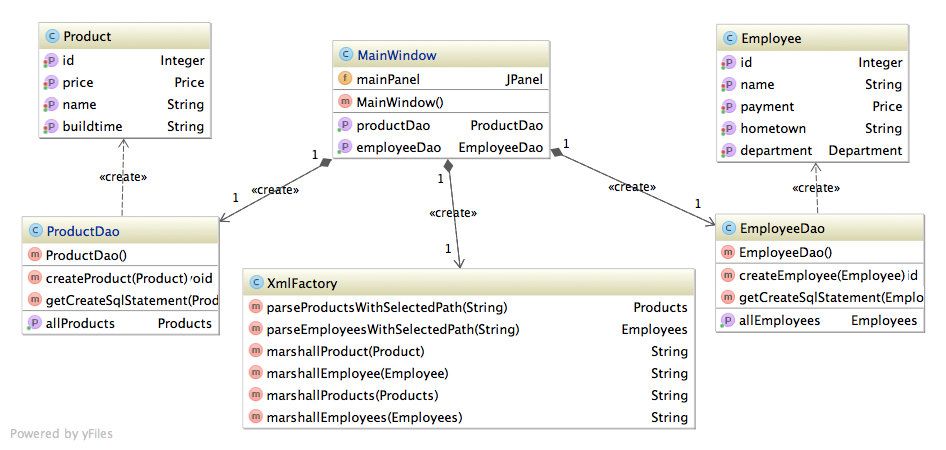
\includegraphics[width=0.95\textwidth ]{class.png}{}
    \centering
    \caption{Klassendiagramm des Parser Projekts}\label{fig:class}
\end{figure*}

In der Abbildung \ref{fig:class} ist das vereinfachte Klassendiagramm des Projekts zu entnehmen, welches den Kommunikationsweg zum Parsen von XML durch \enquote{XmlFactory} und Speichern in die Datenbank durch die \enquote{Dao-Klassen} darstellt. Zur einfachen Ansicht des Parsens und der Datenbankansicht wurde die Hauptklasse als Swing Form verwirklicht. Die Oberfläche ist in Abbildung \ref{fig:app1} und \ref{fig:app2} zu erkennen. 

\begin{figure}[ht]
    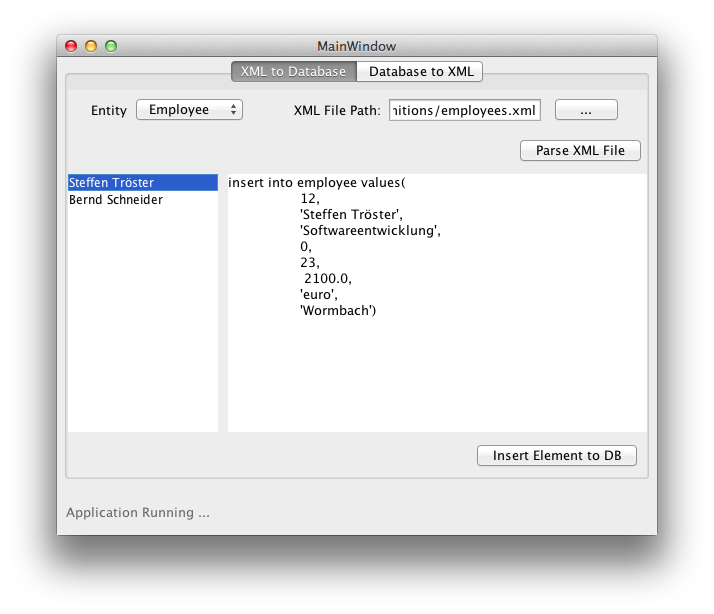
\includegraphics[width=0.5\textwidth ]{app1.png}{}
    \centering
    \caption{XML Parser wandelt XML Instanzen in SQL Statements.}\label{fig:app1}
\end{figure}

\begin{figure}[ht]
    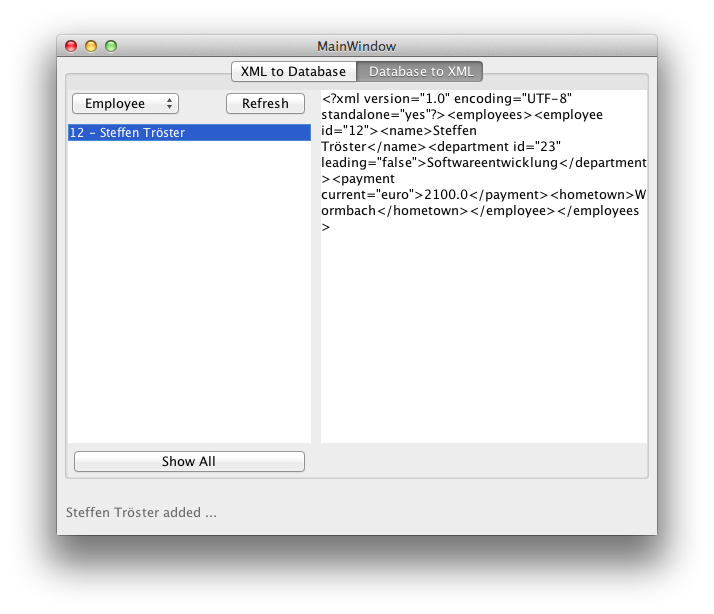
\includegraphics[width=0.5\textwidth ]{app2.png}{}
    \centering
    \caption{Einträge aus der Datenbank werden in XML Dokumente umgewandelt.}\label{fig:app2}
\end{figure}

\section{Ausblick}

Um das Speichern in eine Datenbank abhänig des XML Schemas zu gestalten, müssen die entsprechenden SQL Statements bei Änderungen des Schemas manuell angepasst werden. Diesen Schritt könnte man durch ein \enquote{Objekt-Relationales-Mapping (ORM)} überspringen, sodass bei Schemaänderungen und dem Generieren von Domänenklassen auch automatisch das Schema der Datenbank angepasst wird. Die Java-Bibliotheken JPA könnte da mittels Hibernate oder Ebean zum Einsatz kommen.  \\

\bibliography{references}


\end{document}





